\documentclass{beamer}

\usepackage[utf8]{inputenc}
\usepackage[T1]{fontenc}
\usepackage{amsmath}
\usepackage{amssymb}
\usepackage{amsthm}
\usepackage{graphicx}
\usepackage{hyperref}
\usepackage{booktabs}
\usepackage{bm}
\usepackage{enumerate}
\usepackage{tikz}
\usepackage{subcaption}
\usepackage{lmodern} % For better font rendering

\usetheme{Antibes}
\usecolortheme{default}

\title{Analysis of the Neural Tangent Hierarchy and the First-Order Correction Kernel $K^{(3)}$}
\subtitle{Theory, Scaling, and Experiments}
\author{Janis Aiad}
\institute{UMD, Ecole Polytechnique}
\date{\today}

% Math commands from report
\newcommand{\E}{\mathbb{E}}
\newcommand{\R}{\mathbb{R}}
\newcommand{\N}{\mathbb{N}}
\newcommand{\C}{\mathbb{C}}
\newcommand{\I}{\mathbf{I}}
\newcommand{\norm}[1]{\left\lVert#1\right\rVert}
\newcommand{\abs}[1]{\left\lvert#1\right\rvert}
\newcommand{\evmin}[1]{\lambda_{\min}\left(#1\right)}
\newcommand{\evmax}[1]{\lambda_{\max}\left(#1\right)}
\newcommand{\svmin}[1]{\sigma_{\min}\left(#1\right)}
\newcommand{\tr}{\text{tr}}
\newcommand{\x}{\mathbf{x}}
\newcommand{\g}{\mathbf{g}}
\newcommand{\y}{\mathbf{y}}
\newcommand{\f}{\mathbf{f}}
\newcommand{\Ktwo}{K^{(2)}}
\newcommand{\Kthree}{K^{(3)}}
\newcommand{\Order}{\mathcal{O}}

\begin{document}

\begin{frame}
\titlepage
\end{frame}

\begin{frame}{Outline}
\tableofcontents
\end{frame}

\section{Introduction: Beyond Infinite Width}

\begin{frame}{The Success and Limits of the NTK}
\textbf{The Neural Tangent Kernel (NTK):}
\begin{itemize}
    \item A major breakthrough for understanding training dynamics of neural networks.
    \item In the infinite-width limit, the NTK ($K^{(2)}$) becomes a fixed kernel.
    \item Training dynamics simplify to kernel regression, a convex optimization problem.
\end{itemize}
\vspace{1cm}
\textbf{The Finite-Width Gap:}
\begin{itemize}
    \item Real-world, finite-width networks often outperform their infinite-width counterparts.
    \item This suggests that finite-width effects, like the \textit{evolution of the NTK during training}, are crucial for performance.
\end{itemize}
\end{frame}

\begin{frame}{Our Goal: Understanding the First Correction}
To study finite-width effects, we turn to the \textbf{Neural Tangent Hierarchy (NTH)}.
\begin{itemize}
    \item The NTH describes dynamics as a hierarchy of coupled ODEs.
    \item The evolution of the network output $f$ is governed by $K^{(2)}$.
    \item The evolution of $K^{(2)}$ is governed by a third-order kernel, $K^{(3)}$.
\end{itemize}
\vspace{1cm}
\textbf{In this presentation, we will:}
\begin{enumerate}
    \item Formally derive the expression for the first-order correction kernel, $K^{(3)}$.
    \item Analyze how its magnitude scales with network depth ($H$) and width ($m$).
    \item Present numerical experiments that validate our theoretical findings.
\end{enumerate}
\end{frame}

\section{The Neural Tangent Hierarchy}

\begin{frame}{From NTK to the Hierarchy}
The dynamics of the network output $f_\alpha(t) := f(x_\alpha, \theta_t)$ are given by:
\[
\frac{d f_\alpha(t)}{dt} = -\frac{1}{n} \sum_{\beta=1}^n K^{(2)}_t(x_\alpha, x_\beta) (f_\beta(t) - y_\beta)
\]
\begin{definition}[Neural Tangent Kernel]
$K^{(2)}_t(x_\alpha, x_\beta) := \langle \nabla_\theta f_t(x_\alpha), \nabla_\theta f_t(x_\beta) \rangle$
\end{definition}
\vspace{0.5cm}

\begin{definition}[Third-Order Kernel]
$K^{(3)}_t(x_\alpha, x_\beta, x_\gamma) := \langle \nabla_\theta K^{(2)}_t(x_\alpha, x_\beta), \nabla_\theta f_t(x_\gamma) \rangle$
\end{definition}
This defines an infinite hierarchy where the dynamics of $K^{(r)}$ are governed by $K^{(r+1)}$.
\end{frame}

\begin{frame}{The NTK Spectrum at Infinite Width}
\textbf{The spectrum of the infinite-width NTK has a distinct structure:}
\begin{itemize}
    \item There is one large, isolated eigenvalue that remains constant with depth.
    \item The rest of the eigenvalues form a "bulk" that scales linearly with depth $L$ (as $\sim 0.75 L/N$).
    \item This linear scaling of the small eigenvalues is what amplifies the finite-width corrections in deep networks.
\end{itemize}

\begin{columns}[T] % Aligns top of columns
\column{0.5\textwidth}
    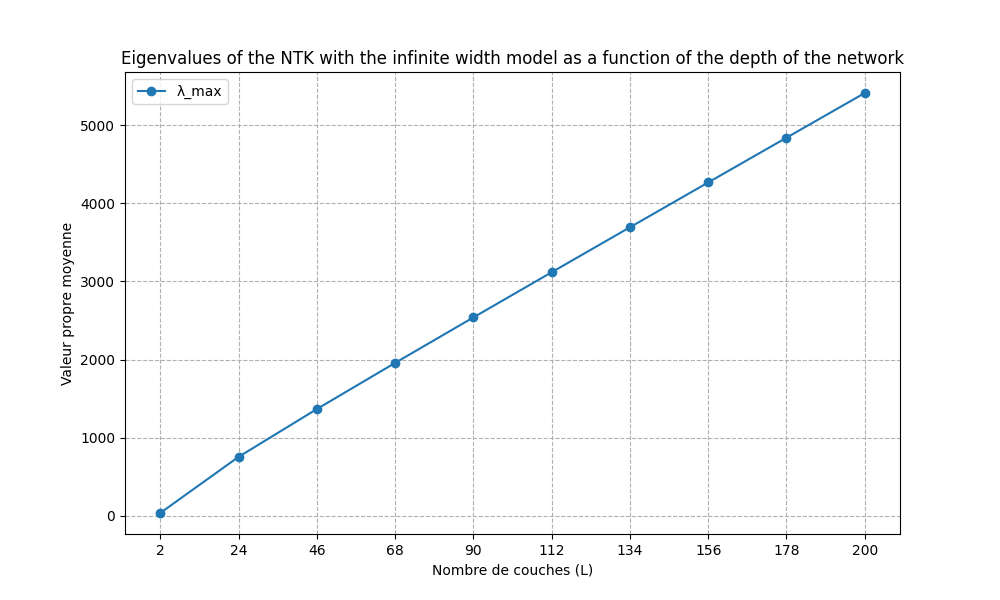
\includegraphics[width=\textwidth]{largest_eigenvalue_vs_L_infinite.png}
    \captionof{figure}{\tiny Largest eigenvalue vs. Depth L.}

\column{0.5\textwidth}
    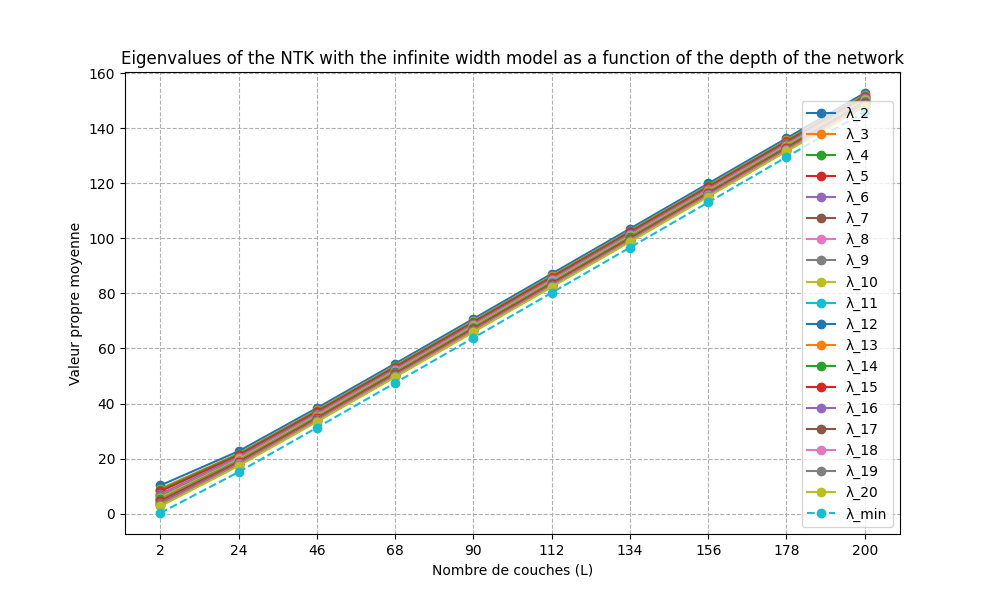
\includegraphics[width=\textwidth]{kth_eigenvalue_vs_L_infinite.png}
    \captionof{figure}{\tiny Smallest eigenvalues vs. Depth L.}
\end{columns}

\textbf{Interpretation:}
\begin{itemize}
    \item \textbf{Depth ($L$):} Super-linear growth.
    \item \textbf{Data Size ($N$):} Linear growth.
    \item \textbf{Input Dimension ($D_{in}$):} Bounded dependence. The correction does not grow with input dimension, which is ideal for high-dimensional problems.
    \item \textbf{Width ($M$):} Decays as $\sim 1/M$, as expected from theory.
\end{itemize}

\vfill
\tiny{\textit{Disclaimer: These results are based on extensive computations ($\sim$100h+) and are fully reproducible via the provided codebase.}}

\end{frame}

\begin{frame}{Goal: The Late-Time NTK Correction}
To understand the full impact of the NTK's evolution, we focus on the final, first-order correction after training, $\Theta^{(1)}_\infty$.
\begin{theorem}[Late-Time Correction \cite{large-width-feynman}]
\begin{align*}
\Theta^{(1)}_\infty = & -\sum_{i}\frac{1}{\lambda_{i}}(O_{3}(\vec{x};0)\cdot\hat{e}_{i})(\Delta f_{0}\cdot\hat{e}_{i}) \\
& + \sum_{i,j}\frac{1}{\lambda_{i}(\lambda_{i}+\lambda_{j})}(\hat{e}_{i}^{T}O_{4}(\vec{x};0)\hat{e}_{j})(\Delta f_{0}\cdot \hat{e}_{i})(\Delta f_{0}\cdot \hat{e}_{j})
\end{align*}
\end{theorem}
\vspace{-0.5cm}
\begin{center}
\small
This shows the correction depends on higher-order kernels ($O_3$, $O_4$) and the spectrum ($\lambda_i$).\\ Our first step is to analyze $K^{(3)} \equiv O_3$.
\end{center}
\end{frame}

\section{Deeper Dive: NTK Correction Scaling}

\begin{frame}{Experimental Setup for NTK Correction}
\textbf{Goal:} Empirically measure the full NTK correction and find its scaling law.
\begin{itemize}
    \item \textbf{Setup:} JAX and Neural Tangents library.
    \item \textbf{Measure:} Spectral radius of the scaled correction, $\|M(K_{\text{emp}} - K_{\infty})\|$.
    \item \textbf{Parameters Varied:}
    \begin{itemize}
        \item Depth $L \in [2, 1000]$
        \item Width $M \in [10, 5000]$
        \item Input Dim $D_{in} \in [20, 5000]$
        \item Data Size $N \in [8, 256]$
    \end{itemize}
    \item \textbf{Rigor:} 10 runs per configuration for statistical robustness.
\end{itemize}
\end{frame}

\begin{frame}{Empirical Scaling of the NTK Correction}
A multivariate regression in log-space ($R^2=0.994$) on the correction's spectral radius yields a precise scaling law:

\begin{alertblock}{Empirical Scaling Law}
\[
\|K - K_\infty\| \propto L^{1.171} \cdot D_{\text{in}}^{0.047} \cdot N^{0.900} \cdot M^{-1.009}
\]
\end{alertblock}

\textbf{Interpretation:}
\begin{itemize}
    \item \textbf{Depth ($L$):} Super-linear growth.
    \item \textbf{Data Size ($N$):} Linear growth.
    \item \textbf{Input Dimension ($D_{in}$):} Bounded dependence. The correction does not grow with input dimension, which is ideal for high-dimensional problems.
    \item \textbf{Width ($M$):} Decays as $\sim 1/M$, as expected from theory.
\end{itemize}

\vfill
\tiny{\textit{Disclaimer: These results are based on extensive computations ($\sim$100h+) and are fully reproducible via the provided codebase.}}

\end{frame}

\begin{frame}{Correction Scaling vs. Depth ($L$)}
    \begin{figure}
        \centering
        \includegraphics[width=0.7\textwidth]{spectralradiusallconfigsL.png}
        \caption{Correction's spectral radius vs. depth $L$. This plot aggregates results across all configurations, confirming the super-linear growth trend on a log-log scale, consistent with $L^{1.171}$.}
    \end{figure}
\end{frame}

\begin{frame}{Correction Scaling vs. Data Size ($N$)}
    \begin{figure}
        \centering
        \includegraphics[width=0.7\textwidth]{spectralradiusallconfigsN.png}
        \caption{Correction's spectral radius vs. data size $N$. The trend supports a near-linear scaling ($N^{0.900}$), confirming that the correction becomes more significant for larger datasets.}
    \end{figure}
\end{frame}

\begin{frame}{Correction Scaling vs. Input Dimension ($D_{in}$)}
    \begin{figure}
        \centering
        \includegraphics[width=0.7\textwidth]{spectralradiusallconfigsD.png}
        \caption{Correction's spectral radius vs. input dimension $D_{in}$. The flat trend provides strong evidence that the dependence on dimension is bounded, a crucial result for high-dimensional applications.}
    \end{figure}
\end{frame}


\begin{frame}{Hypothetical Scaling for $\lambda_{\min}$}
\begin{alertblock}{Finite-Width Bound}
Including finite-width effects, we conjecture a more precise bound based on our experiments and Weyl's inequality:
\[ \lambda_{\min}(K_{\text{emp}}) \ge \frac{0.75L}{N} - C \frac{NL}{M} \]
\end{alertblock}
This shows that the finite-width term further decreases the small eigenvalues.
For a parameter budget $P = M^2L$, we first optimize with respect to $L$:
\[
M = \sqrt{\frac{P}{L}} \implies \lambda_{\min} \ge \frac{0.75L}{N} - C \frac{NL}{\sqrt{\frac{P}{L}}} 
\]
\end{frame}

\begin{frame}{Optimal Configuration}
The optimal value of $L$ occurs when the derivative of $\lambda_{\min}$ with respect to $L$ is zero:
\[
\frac{\partial}{\partial L} \lambda_{\min} = \frac{0.75}{N} - \frac{3}{2} C \frac{N}{\sqrt{P}} L^{1/2} = 0 \implies L^* = \frac{0.25 P}{C^2 N^4}
\]

This gives the optimal width:
\[
M^* = \sqrt{\frac{P}{L^*}} = 2 C N^2
\]

These values maximize the lower bound on $\lambda_{\min}$ for a fixed parameter budget $P$ and dataset size $N$.

\end{frame}

\begin{frame}{Important Caveat}
\begin{alertblock}{Important Caveat}
This analysis relies on Weyl's inequality without taking the eigenvalues signs into account, which provides a very loose bound. The actual behavior may differ significantly from these predictions. For more accurate results, we should focus on better estimating the $K^{(3)}$ and $K^{(4)}$ terms directly.
\end{alertblock}
\end{frame}

\section{Derivation of the $K^{(3)}$ Formula}

\begin{frame}{$K^{(3)}$: Structure and Components}
Let $\delta_\gamma(\cdot) := \langle \nabla_\theta (\cdot), \nabla_\theta f_t(x_\gamma) \rangle$. Then $K^{(3)}_{\alpha\beta\gamma} = \delta_\gamma(K^{(2)}_{\alpha\beta})$.
\vspace{0.2cm}
The NTK for an $H$-layer MLP has the form:
\[
K^{(2)}_{\alpha\beta} = \langle x^{(H)}_\alpha, x^{(H)}_\beta \rangle + \sum_{\ell=1}^{H} \langle G^{(\ell)}_\alpha, G^{(\ell)}_\beta \rangle \langle x^{(\ell-1)}_\alpha, x^{(\ell-1)}_\beta \rangle
\]
Applying the product rule for $\delta_\gamma$ yields a decomposition into four main parts:
\begin{align*}
K^{(3)}_{\alpha\beta\gamma} = K^{(3,\text{out})} + K^{(3,G,W)} + K^{(3,G,a)} + K^{(3,x)}
\end{align*}
\begin{itemize}
    \item $K^{(3,\text{out})}$: from derivatives of final layer activations $x^{(H)}$.
    \item $K^{(3,G,W)}$: from derivatives of backward vectors $G^{(\ell)}$ w.r.t. weights $W$.
    \item $K^{(3,G,a)}$: from derivatives of $G^{(\ell)}$ w.r.t. output weights $a$.
    \item $K^{(3,x)}$: from derivatives of hidden layer activations $x^{(\ell-1)}$.
\end{itemize}
\end{frame}

\begin{frame}{Recursive Derivatives}
\begin{proposition}[Recursive Derivatives]
The core of the derivation is to compute the directional derivatives of the activations and backward vectors. They follow these recursions:
\begin{itemize}
    \item \textbf{Forward derivative $\delta_\gamma x^{(p)}$:}
    \[
    \delta_\gamma x^{(p)}_\mu = \frac{\sigma'_{p}}{\sqrt{m}} \left( W^{(p)} (\delta_\gamma x^{(p-1)}_\mu) + \langle x^{(p-1)}_\gamma, x^{(p-1)}_\mu \rangle G^{(p)}_\gamma \right)
    \]
    This recursion accumulates terms at each layer.
    
    \item \textbf{Backward derivative $\delta_\gamma G^{(\ell)}$:}
    \[
    \delta_\gamma G^{(\ell)}_\mu = \text{sum of terms from replacing } W^{(p+1)} \text{ and } a_t
    \]
    This involves summing contributions from all subsequent layers $p > \ell$.
\end{itemize}
\end{proposition}
\end{frame}

\begin{frame}{The Final Formula}
\begin{theorem}[Fully Expanded Formula for $K^{(3)}$ with ReLU]
By unrolling the recursions, we obtain a complete, non-recursive formula for $K^{(3)}$. The full expression is complex, but it is a sum of the four components identified earlier:
\begin{align*}
K^{(3)}_{\alpha\beta\gamma} = K^{(3,\text{out})}_{\alpha\beta\gamma} + K^{(3,G,W)}_{\alpha\beta\gamma} + K^{(3,G,a)}_{\alpha\beta\gamma} + K^{(3,x)}_{\alpha\beta\gamma}
\end{align*}
Each component is an explicit (but lengthy) sum over layers involving activations, backward vectors, and their inner products.
\end{theorem}
\end{frame}

\begin{frame}{$K^{(3)}$: Structure and Components}
\begin{columns}
\column{0.5\textwidth}
\textbf{1. Why linear scaling with L?}
\begin{itemize}
    \item Our experiments showed that the $K^{(3)} \equiv O_3$ kernel's norm diminishes with width.
    \item Therefore, the $O_3$ term's contribution is suppressed.
    \item The observed linear growth of the correction with depth $L$ must be primarily driven by the \textbf{$O_4$ term}.
    \item \textit{Note: The exact scaling of the $O_3$ term is complex and under active experimental investigation.}
\end{itemize}

\column{0.5\textwidth}
\textbf{2. Why scaling with L and N?}
\begin{itemize}
    \item The correction is amplified by small eigenvalues ($\lambda_i$), which we've just seen scale as $\sim L/N$.
    \item A larger $L$ or $N$ means a smaller $\lambda_{\min}$, which \textbf{boosts the correction}, explaining the scaling.
\end{itemize}
\end{columns}
\end{frame}



\begin{frame}{Theoretical Interpretation of the Scaling Law (not sure of that)}
    The late-time NTK correction formula, $\Theta^{(1)}_\infty$, explains our empirical findings.
    
    \begin{columns}
    \column{0.5\textwidth}
    \textbf{1. Why super-linear scaling with L?}
    \begin{itemize}
        \item While $\|K^{(3)}\| \sim \Order(L^2/\sqrt{m})$, experiments show it diminishes with width.
        \item Its contribution to the correction is suppressed.
        \item The observed super-linear growth of the correction with depth $L$ must be primarily driven by the \textbf{$O_4$ term}.
        \item \textit{Note: The exact scaling of the $O_4$ term is a key area for future work.}
    \end{itemize}
    
    \column{0.5\textwidth}
    \textbf{2. Why scaling with L and N?}
    \begin{itemize}
        \item The correction is amplified by small eigenvalues ($\lambda_i$) of the NTK.
        \item We've seen these eigenvalues scale as $\sim L/N$.
        \item A larger $L$ or smaller $N$ means a smaller $\lambda_{\min}$, which \textbf{boosts the correction}, explaining the observed scaling.
    \end{itemize}
    \end{columns}
    \end{frame}


\section{Scaling and Validation of $K^{(3)}$}

\begin{frame}{Theoretical Scaling of Core Components}
\begin{itemize}
    \item \textbf{Activations and G-vectors:}
    With proper initialization (dynamical isometry), norms are stable across layers:
    \[ \|x^{(p)}_\mu\| \sim \Order(1) \quad \text{and} \quad \|G^{(\ell)}_\mu\| \sim \Order(1) \]
    
    \item \textbf{Numerical Challenge: Lyapunov Exponents}
    For any \textit{finite} width, the norm of products of random matrices is governed by Lyapunov exponents. Disentangling potential small exponential trends from the polynomial scaling we want to measure is hard.
    
    \item \textbf{Derivative Terms Scaling:}
    \begin{align*}
    \|\delta_\gamma x^{(p)}_\mu\| &\sim \Order\left(\frac{p}{\sqrt{m}}\right) \quad (\text{linear growth with layer } p) \\
    \|\delta_\gamma G^{(\ell)}_\mu\| &\sim \Order\left(\frac{H-\ell}{m}\right) \quad (\text{grows with number of subsequent layers})
    \end{align*}
\end{itemize}
\end{frame}

\begin{frame}{Term-by-Term and Overall Scaling of $K^{(3)}$}
Combining component scalings gives the scaling of the full tensor.

\begin{columns}
\column{0.6\textwidth}
\textbf{Term-by-term analysis ($H \ll \sqrt{m}$):}
\begin{itemize}
    \item $K^{(3, \text{out})} \sim \Order(H/\sqrt{m})$
    \item $K^{(3, G, W)} \sim \Order(H^2/m)$
    \item $K^{(3, G, a)} \sim \Order(H/\sqrt{m})$
    \item $K^{(3, x)} \sim \Order(H^2/\sqrt{m})$
\end{itemize}
\column{0.4\textwidth}
The forward term $K^{(3,x)}$ dominates the scaling.
\end{columns}

\begin{alertblock}{Overall Scaling of $K^{(3)}$}
The magnitude of the third-order kernel scales as:
\begin{equation*}
K^{(3)}_{\alpha\beta\gamma} \sim \Order\left(\frac{H^2}{\sqrt{m}}\right)
\end{equation*}
\end{alertblock}
This implies finite-width effects grow quadratically with depth.
\end{frame}

\begin{frame}{Experimental Setup for $K^{(3)}$}
\textbf{Goal:} Empirically compute $K^{(3)}$ and verify the $\Order(H^2/\sqrt{m})$ scaling law.
\begin{itemize}
    \item \textbf{Architecture:} MLP with ReLU, varying depth $L$ (same as $H$).
    \item \textbf{Data:} $N=8$ random, normalized data points in $D_{in}=20$.
    \item \textbf{Width:} Fixed at $M=100$.
    \item \textbf{Methodology:}
        \begin{enumerate}
            \item Initialize network for a given depth $L$.
            \item Perform forward pass, storing activations and derivatives.
            \item Compute the full $K^{(3)}$ tensor using the derived formulas.
            \item Calculate its infinity norm $\|K^{(3)}\|_\infty = \max |K^{(3)}_{\alpha\beta\gamma}|$.
        \end{enumerate}
\end{itemize}
\end{frame}

\begin{frame}{Results: $K^{(3)}$ Scaling}
\begin{figure}[h]
    \centering
    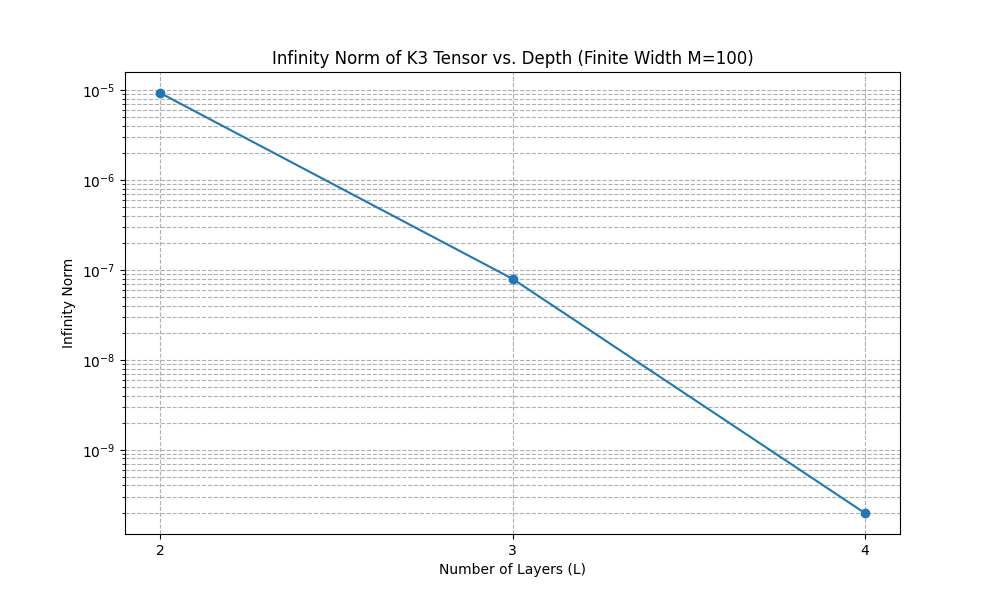
\includegraphics[width=0.8\textwidth]{k3_inf_norm_vs_L_finite_M100_N8_D20.png}
    \caption{Infinity norm of empirical $K^{(3)}$ vs. network depth $L$ (M=100).}
    \label{fig:k3_norm_vs_l}
\end{figure}
\begin{itemize}
    \item The plot clearly shows that the magnitude of $K^{(3)}$ \textbf{grows} with depth.
    \item The trend is strongly consistent with our theoretical prediction $K^{(3)} \sim \Order(L^2/\sqrt{m})$.
    \item This validates that finite-width effects become more pronounced in deeper networks.
\end{itemize}
\end{frame}

\section{Future Work}
\begin{frame}{Future Work}
\begin{itemize}
    \item \textbf{Neural Tangent Hierarchy:}
    \begin{itemize}
        \item Compute scaling of hierarchical coefficients ($\lambda_H$)
        \item Empirically verify predicted linear scaling with depth
    \end{itemize}
    
    \item \textbf{$O_4$ Kernel Analysis:}
    \begin{itemize}
        \item Study detailed properties and eigendecomposition
        \item Develop full implementation if not available in literature
        \item Analyze structure and contribution to feature learning
    \end{itemize}
    
    \item \textbf{Generalization:}
    \begin{itemize}
        \item Extend numerical framework to structured data
        \item Test on torus and over $\mathbb{R}^d$
    \end{itemize}
    
    \item \textbf{Modern Architectures:}
    \begin{itemize}
        \item Bridge theory-practice gap
        \item Expand analysis to complex architectures like ResNets
    \end{itemize}
\end{itemize}
\end{frame}

\section{Conclusion}

\begin{frame}{Conclusion}
\textbf{Summary:}
\begin{itemize}
    \item We moved beyond the infinite-width NTK by analyzing the NTH.
    \item We derived a complete formula for the first-order correction kernel, $K^{(3)}$.
    \item We showed theoretical insights and empirical results for the 1/M scaling of the correction term.
\end{itemize}
\vspace{1cm}
\textbf{Key Implication:}
\begin{alertblock}
The training dynamics of deep networks are inherently richer than shallow ones. The learning geometry itself (the NTK) evolves more significantly, meaning deep networks are less "lazy". This provides a theoretical basis for their powerful feature learning capabilities.
\end{alertblock}
\end{frame}

\end{document}
